\documentclass[11pt,a4paper,twoside]{article}
\usepackage[margin=1.2cm]{geometry}
\usepackage{multicol}
\usepackage{amsmath, amssymb}
\usepackage{tikz}
\usetikzlibrary{automata, positioning, calc}
\setlength{\columnsep}{-3cm}
\raggedcolumns%
\newcommand\blank[1][.6em]{%
  \makebox[#1]{%
    \kern.07em
    \vrule height.3ex
    \hrulefill%
    \vrule height.3ex
    \kern.07em
  }%
}
\newcommand{\transition}[5]{\delta(#1,#2) &= (#3,#4,#5)}
\newcommand{\true}{\mathrm{true}}
\newcommand{\false}{\mathrm{false}}
\newcommand{\id}{\mathrm{id}}
\newcommand{\pred}{\mathrm{pred}}
\newcommand{\numeral}[1]{\overline{#1}}
\begin{document}

\begin{enumerate}
  \item % 1
  \begin{enumerate}
    \item % a
		\begin{figure}[!h] \centering
    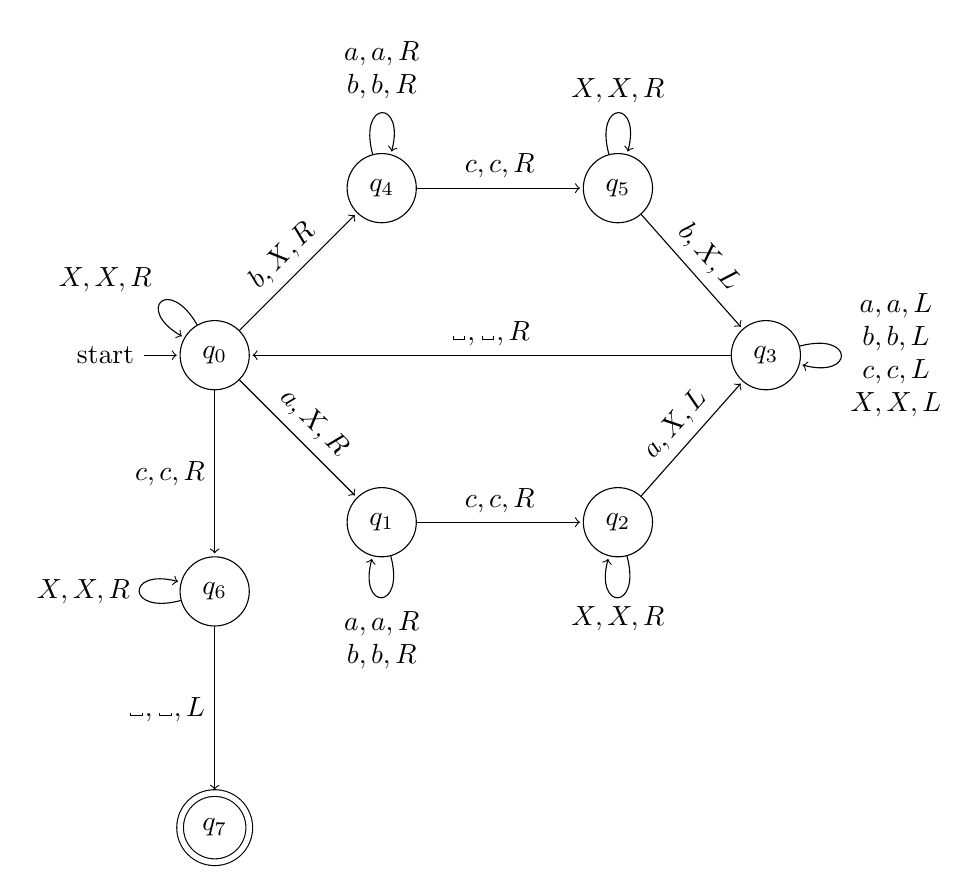
\begin{tikzpicture}[shorten >=1pt, node distance=3cm, on grid, auto]
		\node[state, initial] (0) {$q_0$};
		\node[state]          (1) [below right=of 0] {$q_1$};
		\node[state]          (2) [right=of 1] {$q_2$};
		\node[state]          (3) [right=7cm of 0] {$q_3$};
		\node[state]          (4) [above right=of 0] {$q_4$};
		\node[state]          (5) [right=of 4] {$q_5$};
    \node[state]          (6) [below=of 0] {$q_6$};
    \node[state, double distance=2pt] (7) [below=of 6] {$q_7$};
    \path[->]
      (0) edge [in=150, out=120, loop] node [above left] {$X,X,R$} (0)
      (0) edge               node [pos=0.5, sloped, above] {$a,X,R$} (1)
      (1) edge [loop below]  node {$\begin{matrix}a,a,R\\b,b,R\end{matrix}$} (1)
      (1) edge               node {$c,c,R$} (2)
      (2) edge [loop below]  node {$X,X,R$} (2)
      (2) edge               node [pos=0.5, sloped, above] {$a,X,L$} (3)
      (4) edge [loop above]  node {$\begin{matrix}a,a,R\\b,b,R\end{matrix}$} (4)
      (4) edge               node {$c,c,R$} (5)
      (5) edge               node [pos=0.5, sloped, above] {$b,X,L$} (3)
      (3) edge [loop right]  node {$\begin{matrix}a,a,L\\b,b,L\\c,c,L\\X,X,L\end{matrix}$} (3)
      (3) edge               node [above] {$\blank,\blank,R$} (0)
      (0) edge               node [pos=0.5, sloped, above] {$b,X,R$} (4)
      (5) edge [loop above]  node {$X,X,R$} (5)
      (0) edge [left]        node {$c,c,R$} (6)
      (6) edge [loop left]   node {$X,X,R$} (6)
      (6) edge [left]        node {$\blank,\blank,L$} (7);
    \end{tikzpicture}
		\end{figure}

    \begin{multicols}{2}
      \item % b
      $\begin{aligned}[t]
        (\epsilon, q_0, bacbba)
          &\vdash (X,    q_4, acbba) \\
          &\vdash (Xa,   q_4, cbba) \\
          &\vdash (Xac,  q_5, bba) \\
          &\vdash (Xa,   q_3, cXba) \\
          &\vdash (X,    q_3, acXba) \\
          &\vdash (\epsilon,    q_3, XacXba) \\
          &\vdash (\epsilon,    q_3, \blank XacXba) \\
          &\vdash (\epsilon,    q_0, XacXba) \\
          &\vdash (X,    q_0, acXba) \\
          &\vdash (XX,   q_1, cXba) \\
          &\vdash (XXc,  q_2, Xba) \\
          &\vdash (XXcX, q_2, ba) \\
          &\mathrm{Rejected}
      \end{aligned}$

      \item % c
      \centering
      $\begin{aligned}[t]
        (\epsilon, q_0, abcab)
          &\vdash (X,     q_1, bcab) \\
          &\vdash (Xb,    q_1, cab) \\
          &\vdash (Xbc,   q_2, ab) \\
          &\vdash (Xb,    q_3, cXb) \\
          &\vdash (X,     q_3, bcXb) \\
          &\vdash (\epsilon,     q_3, XbcXb) \\
          &\vdash (\epsilon,     q_3, \blank XbcXb) \\
          &\vdash (\epsilon,     q_0, XbcXb) \\
          &\vdash (X,     q_0, bcXb) \\
          &\vdash (XX,    q_4, cXb) \\
          &\vdash (XXc,   q_5, Xb) \\
          &\vdash (XXcX,  q_5, b) \\
          &\vdash (XXc,   q_3, XX) \\
          &\vdash (XX,    q_3, cXX) \\
          &\vdash (X,     q_3, XcXX) \\
          &\vdash (\epsilon,     q_3, \blank XXcXX) \\
          &\vdash (\epsilon,     q_0, XXcXX) \\
          &\vdash (X,     q_0, XcXX) \\
          &\vdash (XX,    q_0, cXX) \\
          &\vdash (XXc,   q_6, XX) \\
          &\vdash (XXcX,  q_6, X) \\
          &\vdash (XXcXX, q_6, \epsilon) \\
          &\vdash (XXcX,  q_7, X) \\
          &\mathrm{Accepted}
      \end{aligned}$
    \end{multicols}

    \pagebreak
    \item % d
      Turing machine $M$ accepts words that contain the same sub-word, made up
      of $a$ and $c$ symbols, on both sides of a $c$ symbol. \
      I.e. $xcx$ where $x \in \{ab\}^*$
  \end{enumerate}

  \item % 2
  \begin{enumerate}
    \item % a
		\begin{figure}[!h] \centering
    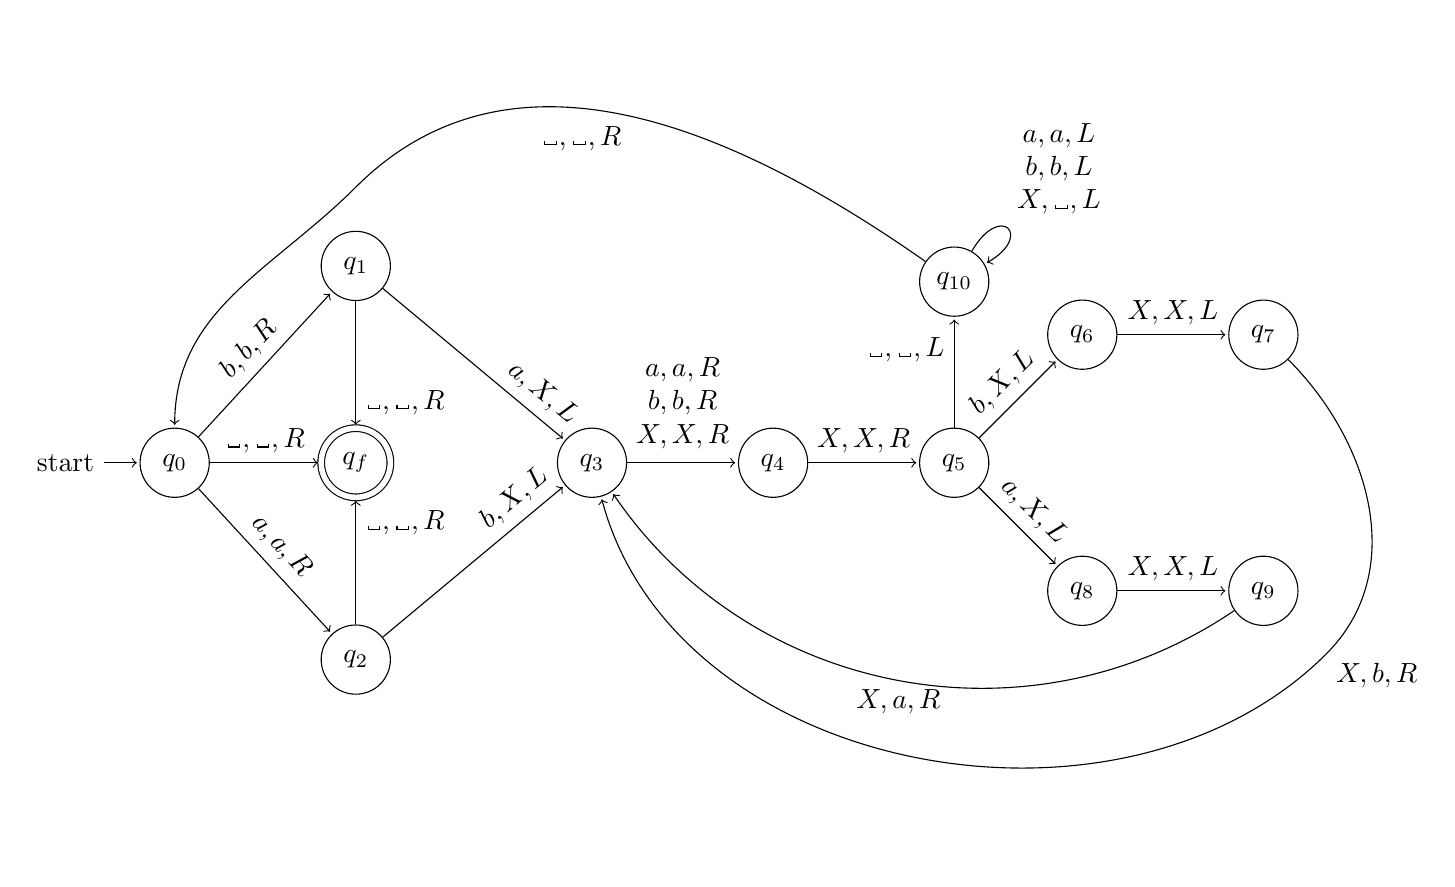
\begin{tikzpicture}[shorten >=1pt, node distance=2.3cm, on grid, auto]
		\node[state, initial] (0) {$q_0$};
    \node[state, double distance=2pt] (f) [right=of 0] {$q_f$};
		\node[state]          (1) [above=2.5cm of f] {$q_1$};
		\node[state]          (2) [below=2.5cm of f] {$q_2$};
		\node[state]          (3) [right=3cm of f] {$q_3$};
		\node[state]          (4) [right=of 3] {$q_4$};
		\node[state]          (5) [right=of 4] {$q_5$};
    \node[state]          (6) [above right=of 5] {$q_6$};
    \node[state]          (7) [right=of 6] {$q_7$};
    \node[state]          (8) [below right=of 5] {$q_8$};
    \node[state]          (9) [right=of 8] {$q_9$};
    \node[state]          (10) [above=of 5] {$q_{10}$};
    \path[->]
      (0) edge node {$\blank,\blank,R$} (f)
      (0) edge node [sloped, above] {$b,b,R$} (1)
      (0) edge node [sloped, above]{$a,a,R$} (2)
      (1) edge node [pos=.8] {$\blank,\blank,R$} (f)
      (2) edge node [right, pos=.8] {$\blank,\blank,R$} (f)
      (1) edge node [sloped, above, pos=.8] {$a,X,L$} (3)
      (2) edge node [sloped, above, pos=.8] {$b,X,L$} (3)
      (3) edge node {$\begin{matrix}a,a,R\\b,b,R\\X,X,R\end{matrix}$} (4)
      (4) edge node {$X,X,R$} (5)
      (5) edge node [sloped, above] {$b,X,L$} (6)
      (5) edge node [sloped, above] {$a,X,L$} (8)
      (5) edge node [pos=.7] {$\blank,\blank,L$} (10)
      (6) edge node {$X,X,L$} (7)
      (8) edge node {$X,X,L$} (9)
      (9) edge [bend left=45] node [below, out=45] {$X,a,R$} (3)
      (10) edge [in=30, out=60, loop] node {$\begin{matrix}a,a,L\\b,b,L\\X,\blank,L\end{matrix}$} (10);

    \draw[->]
      (7) to[out=-45, in=45] ($(9)+(.8cm,-.8cm)$) node [below right] {$X,b,R$} to[in=-75, out=-135] (3);
    \draw[->]
      (10) to[out=145, in=45] node {$\blank,\blank,R$} ($(1)+(0,1cm)$)  to[in=90, out=-135] (0);
    \end{tikzpicture}
		\end{figure}

    \item %b
    \begin{align*}
      M = (Q,\Sigma,\Gamma,\delta,q_0,\blank,F) \quad \mathrm{where} \quad
        Q &= \{q_0,q_1,q_2,q_3,q_4,q_5,q_6,q_7,q_8,q_9,q_{10},q_f\} \\
        F &= \{q_f\} \\
        \Sigma &= \{a,b\} \\
        \Gamma &= \{a,b,X,\blank\} \\
    \end{align*}
    \begin{multicols}{2}
    \begin{align*}
      \transition{q_0}{\blank}{q_f}{\blank}{R} \\
      \transition{q_0}{b}{q_1}{b}{R} \\
      \transition{q_0}{a}{q_2}{a}{R} \\
      \transition{q_1}{\blank}{q_f}{\blank}{R} \\
      \transition{q_1}{b}{q_1}{b}{R} \\
      \transition{q_1}{a}{q_3}{X}{L} \\
      \transition{q_2}{a}{q_2}{a}{R} \\
      \transition{q_2}{\blank}{q_f}{\blank}{R} \\
      \transition{q_2}{b}{q_3}{X}{L} \\
      \transition{q_3}{x}{q_4}{X}{R} \ \mathrm{for} \ x \in \{a,b,X\} \\
    \end{align*}

    \begin{align*}
      \transition{q_4}{X}{q_5}{X}{R} \\
      \transition{q_5}{b}{q_6}{X}{L} \\
      \transition{q_5}{a}{q_8}{X}{L} \\
      \transition{q_5}{a}{q_{10}}{X}{L} \\
      \transition{q_6}{X}{q_7}{X}{L} \\
      \transition{q_7}{X}{q_3}{b}{R} \\
      \transition{q_8}{X}{q_9}{a}{R} \\
      \transition{q_9}{X}{q_3}{a}{R} \\
      \transition{q_{10}}{x}{q_{10}}{x}{L} \ \mathrm{for} \ x \in \{a,b\} \\
      \transition{q_{10}}{X}{q_{10}}{\blank}{L} \\
      \transition{q_{10}}{\blank}{q_0}{\blank}{\blank} \\
    \end{align*}
  \end{multicols}
  \end{enumerate}

  \pagebreak
  \item % 3
  \begin{enumerate}
    \item % a
    \begin{multicols}{2}
    \begin{align*}
      \false\ \id &= \lambda x. \lambda y. y\ \id \\
                  &\leadsto \lambda y. y \\
                  &=_\alpha \lambda x. x \\
                  &= \id \\
      \smallskip \\
      \false\ \true &= \lambda x. \lambda y. y\ \true \\
                    &\leadsto \lambda y. y \\
                    &=_\alpha \lambda x. x \\
                    &= \id \\
      \smallskip \\
      \false\ \false &= \lambda x. \lambda y. y\ \false \\
                     &\leadsto \lambda y. y \\
                     &=_\alpha \lambda x. x \\
                     &= \id \\
    \end{align*}
    \vfill

    \begin{align*}
      \true\ \false &= \lambda x. \lambda y. x\ \false \\
                    &\leadsto \lambda y. \false \\
      \smallskip \\
      \true\ \true &= \lambda x. \lambda y. x\ \true \\
                   &\leadsto \lambda y. \true \\
    \end{align*}
    \vfill
    \end{multicols}

    \item % b
      \begin{align*}
        \mathrm{tidit} \ \numeral{3}
          &= \lambda n. n \ \true\ \id\ \numeral{3} \\
          &\leadsto \numeral{3} \ \true\ \id \\
          &= \lambda f. \lambda x. f\ (f\ (f\ x))\ \true\ \id \\
          &\leadsto \lambda x. \true\ (\true\ (\true\ x))\ \id \\
          &\leadsto \true\ (\true\ (\true\ \id)) \\
          &\leadsto \true\ (\true\ (\lambda y.\id)) \\
          &\leadsto \true\ (\lambda y.\ (\lambda y.\id)) \\
          &\leadsto \lambda y.\ (\lambda y.\ (\lambda y.\id)) \\
          &= \lambda y.\lambda y.\lambda y.\id \\
      \end{align*}

    \item %c
      tidit $\numeral{n}$ drops $n$ arguments provided to it. \\
      Given $n+1$ arguments, it will return the last argument.
  \end{enumerate}

  \item % 4
  \begin{enumerate}
    \item % a
      A Church numeral that is not $\numeral{0}$ will apply the given function at
      least once.\\
      As such, if  $\lambda u.\false$  is provided as the function, and true
      provided as the value, a non $\numeral{0}$ numeral would return false, while
      $\numeral{0}$ would return true.\\
      Thus:\\
      \begin{equation*}
        \mathrm{isZero} = \lambda i. (\lambda u.\false)\ \true
      \end{equation*}

    \item % b
      The predicate of a Church numeral $\numeral{n}$ applies a function
      $n-1$ times.\\
      In order to return an expression that does this,  $\lambda g.\lambda h.h\ (g\ f)$
      can be applied to $\lambda u.x$, which will which will discard a single
      function application.\\
      In order to remove the initial $\lambda h.h$ that would remain at the start
      of the function, the id function is applied.
      Thus:\\
      \begin{equation*}
        \pred = \lambda n.\lambda f. \lambda x. n\ (\lambda g.\lambda h.h\ (g\ f)) (\lambda u.x) (\lambda u.u)
      \end{equation*}

    \item % b
      $n \geq m$ implies that $m-n$ is either zero or negative.\\
      Subtraction can be defined by applying pred a desired number of times:
      \begin{align*}
        \mathrm{sub} = \lambda x.\lambda y.y\ \pred\ x
      \end{align*}
      Since pred cannot result in a `negative' Church numeral, one can simply
      check whether the result of $\mathrm{sub}\ m\ n$ is zero:
      \begin{align*}
        \mathrm{greq}
          &= \lambda n.\lambda m.\mathrm{isZero}\ (\mathrm{sub}\ m\ n) \\
          &= \lambda n.\lambda m.\mathrm{isZero}\ ((\lambda x.\lambda y.y\ \pred\ x)\ m\ n) \\
          &\leadsto \lambda n.\lambda m.\mathrm{isZero}\ (m\ \pred\ n) \\
      \end{align*}

  \end{enumerate}
\end{enumerate}
\end{document}
